\documentclass{standalone}
\usepackage{amsmath}
\usepackage[dvipsnames]{xcolor}
\usepackage{tikz} 
\usetikzlibrary{arrows, decorations.markings,decorations.pathreplacing,angles,quotes}
\usepackage{microtype}
\usepackage{fourier}

\definecolor{py_blue}{rgb}{0.12156862745098039, 0.4666666666666667, 0.7058823529411765}
\definecolor{py_orange}{rgb}{1.0, 0.4980392156862745, 0.054901960784313725}
\definecolor{py_green}{rgb}{0.17254901960784313, 0.6274509803921569, 0.17254901960784313}
\definecolor{py_red}{rgb}{0.8392156862745098, 0.15294117647058825, 0.1568627450980392}
\definecolor{py_purple}{rgb}{0.5803921568627451, 0.403921568627451, 0.7411764705882353}

\begin{document}

\begin{tikzpicture}
	\node[anchor=south west,inner sep=0] (Bild) at (0,0) {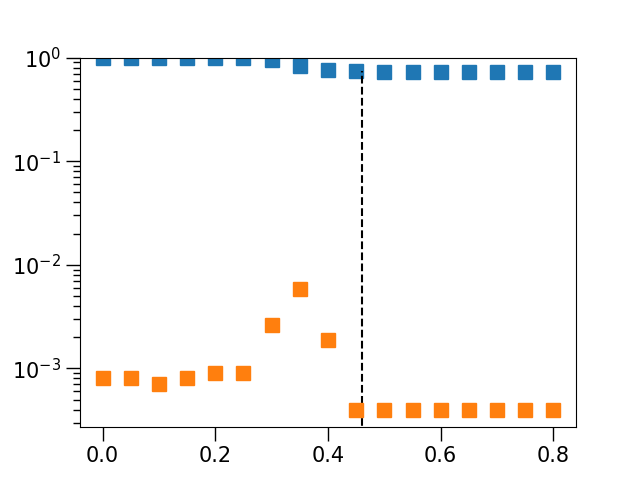
\includegraphics[scale=0.39]{day_read_low_blank}};
   		\begin{scope}[x=(Bild.south east),y=(Bild.north west)]
   			\node (B2) at ([xshift=2.75cm]Bild.east) {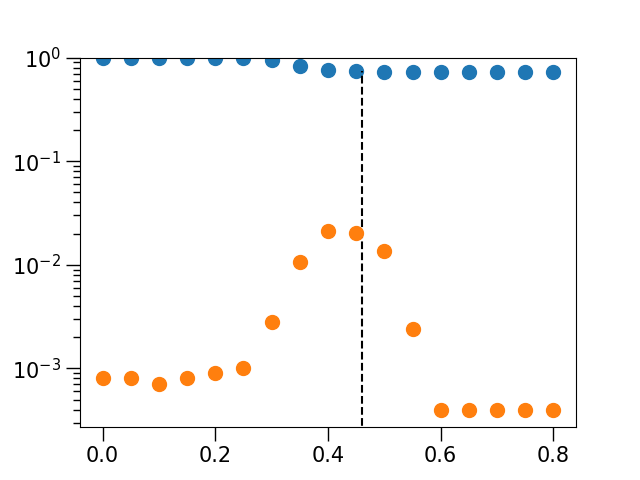
\includegraphics[scale=0.39]{day_read_high_blank}};
                	
        	\node at ([yshift=-.2cm,xshift=-3cm]B2.south) {\large antibiotic concentration $c$};
        	\node[rotate=90] at ([xshift=-.6cm,yshift=-0cm]Bild.west) {emergence/establishment};
        	\node[rotate=90] at ([xshift=-.25cm,yshift=-0cm]Bild.west) {probability};
        	\node at ([yshift=-.2cm]Bild.north) {\large $h_R = 0.45$};
        	\node at ([yshift=-.3cm]B2.north) {\large $h_R=0.6$};
        		
			\node[right=0pt] at (0.14,0.7) {\small \color{py_blue} $\blacksquare$ \color{black} emergence};         	
			\node[right=0pt] at (0.14,0.6) {\small \color{py_orange} $\blacksquare$ \color{black} establishment} (0.2,0.7);    
			\draw[thick,dashed] (0.15,0.5) -- node[right=5pt] {\small \color{black} mic$_S$} (0.2,0.5);  
			
			%\node at ([xshift=.6cm,yshift=1.5cm]Bild.center) {\small msw};   
 			
    	\end{scope}
\end{tikzpicture}

\end{document}